\clearpage
\cqusetheader{3 图表、公式格式}
\section{图表、公式格式}
\subsection{图表格式}
本章将主要介绍一些图表和公式的格式...\\

\begin{figure}[htb]
    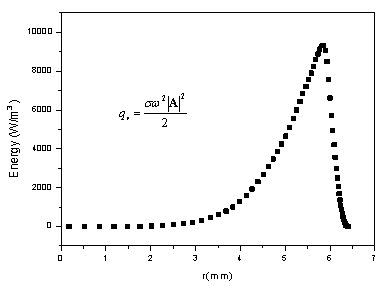
\includegraphics[width=0.9\textwidth]{static/temp.PNG}
    \caption{内热源沿径向的分布}
\end{figure}

\begin{table}[htbp]
    \caption{高频感应加热的基本参数}
    \small
    \begin{tabular}{c c c c}
    \toprule
    感应频率 &感应发生器功率 & 工件移动速度  &感应圈与零件间隙\\
    （KHz）&($\% \times$80Kw) &(mm/min)  &(mm)\\
    \midrule
    250 &88 &5900 &1.65\\
    250 &88 &5900 &1.65\\
    250 &88 &5900 &1.65\\
    250 &88 &5900 &1.65\\
    \bottomrule
    \end{tabular}
\end{table}

\begin{table}[htbp]
    \captionsetup{singlelinecheck=off}
    \caption*{续表3.1}
    \small
    \begin{tabular}{c c c c}
    \toprule
    感应频率 &感应发生器功率 & 工件移动速度  &感应圈与零件间隙\\
    （KHz）&($\% \times$80Kw) &(mm/min)  &(mm)\\
    \midrule
    250 &88 &5900 &1.65\\
    250 &88 &5900 &1.65\\
    \bottomrule
    \end{tabular}
\end{table}


\subsection{公式格式}


\begin{eqnarray}
\frac{1}{\mu} \nabla^2A - j \omega \sigma A -\nabla(\frac{1}{\mu}) \times(\nabla \times A)+J_0=0
\end{eqnarray}


\subsection{本章小结}
本章介绍了……
